\subsection{Ερώτημα iii}
   Ακολουθούν διαγράμματα για το μέγεθος του επεξεργαστή και κατανάλωση ενέργειας.    
   \\\\\\
   \begin{minipage}{\textwidth}
      \begin{center}
         \fbox{\textlatin{\textbf{\textit{Chip Area}}}}\\
         \vspace{3mm}
         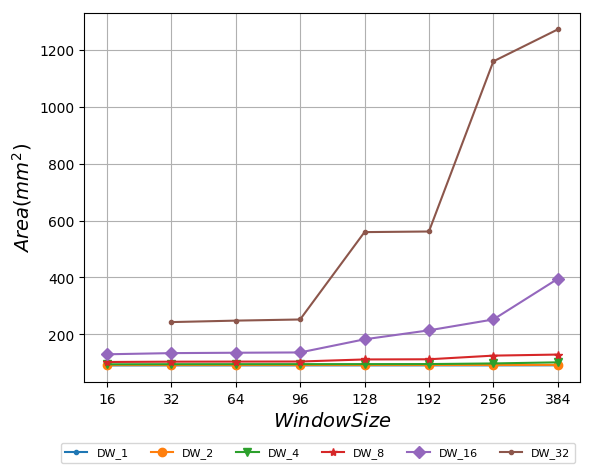
\includegraphics[width=0.7\textwidth]{./graphs/area/area.png}
         \vspace{6mm}
      \end{center}
   \end{minipage}

   \begin{minipage}{\textwidth}
      \begin{center}
         \fbox{\textlatin{\textbf{\textit{403-gcc}}}}\\
         \vspace{3mm}
         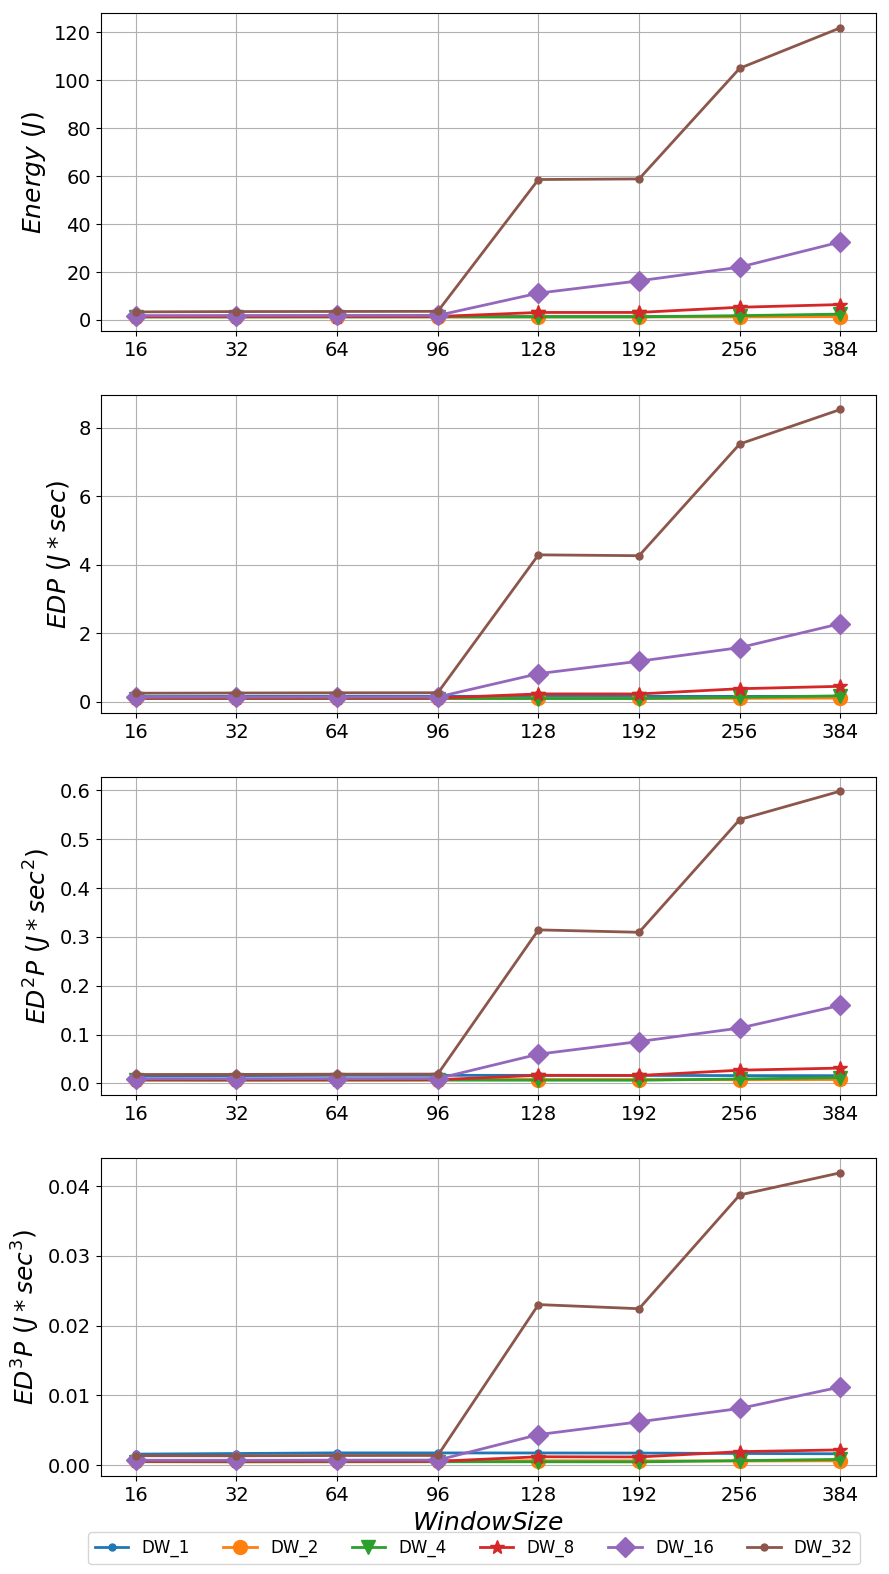
\includegraphics[width=0.7\textwidth]{./graphs/edp/gcc.png}
         \vspace{6mm}
      \end{center}
   \end{minipage}

   \begin{minipage}{\textwidth}
      \begin{center}
         \fbox{\textlatin{\textbf{\textit{429-mcf}}}}\\
         \vspace{3mm}
         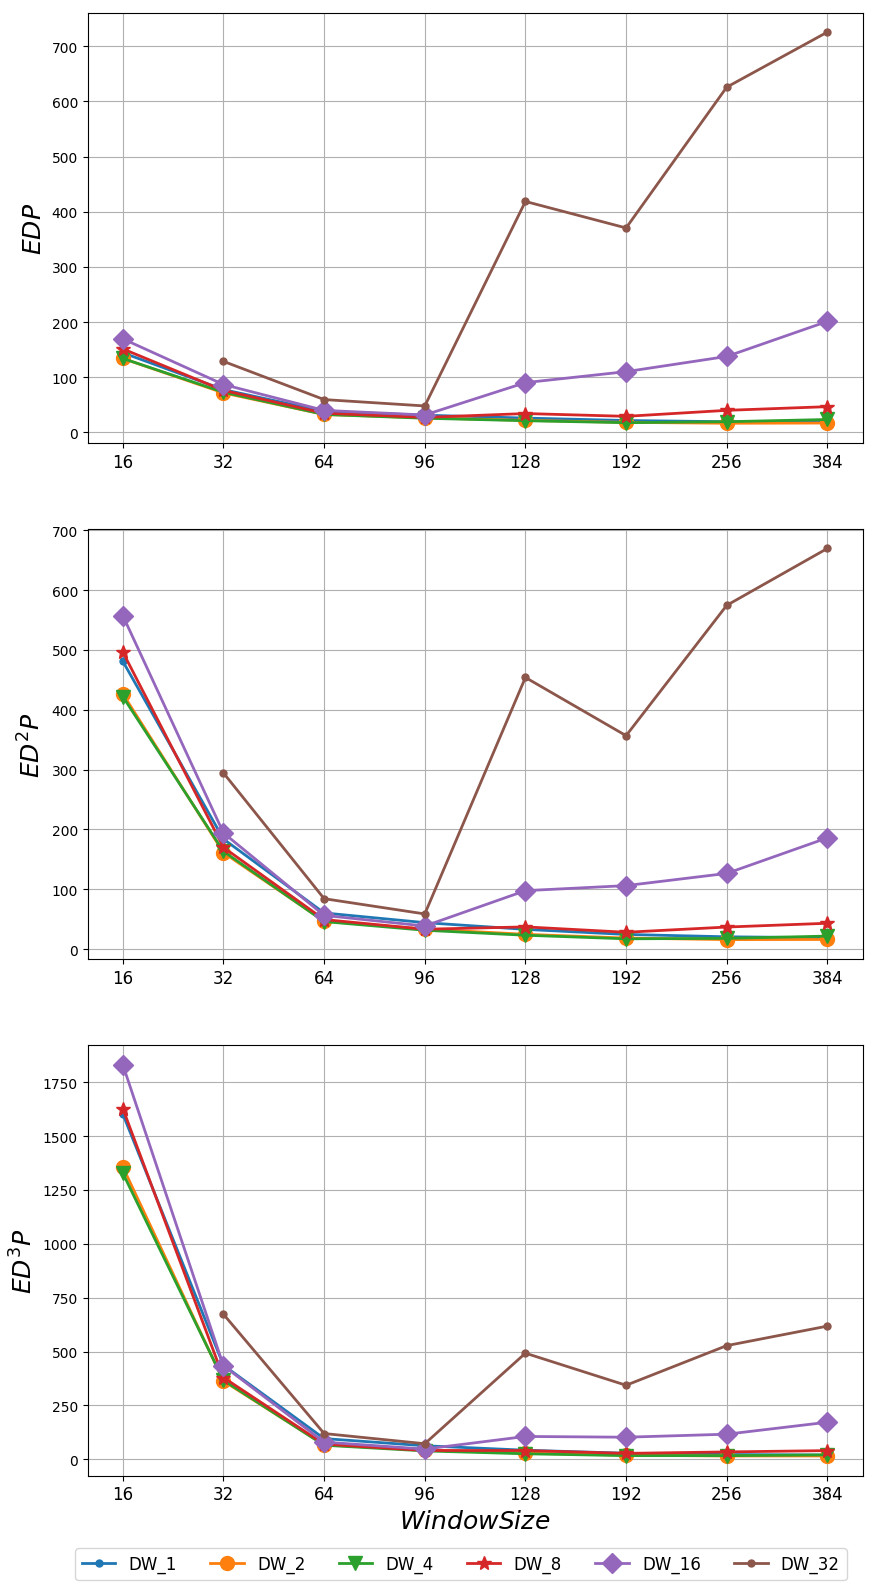
\includegraphics[width=0.7\textwidth]{./graphs/edp/mcf.png}
         \vspace{6mm}
      \end{center}
   \end{minipage}

   \begin{minipage}{\textwidth}
      \begin{center}
         \fbox{\textlatin{\textbf{\textit{434-zeusmp}}}}\\
         \vspace{3mm}
         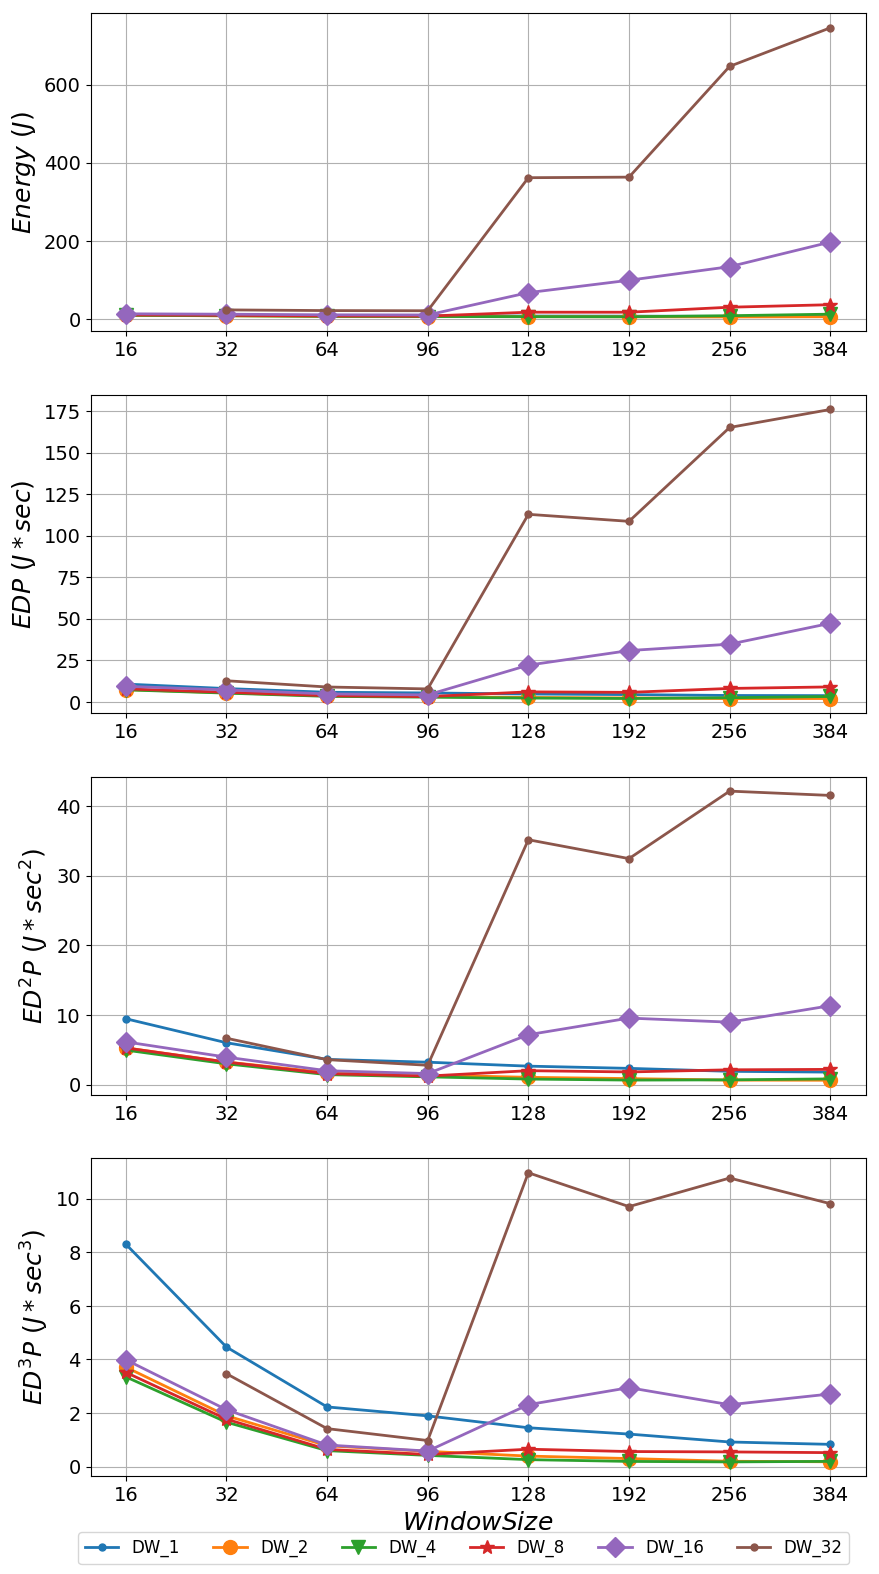
\includegraphics[width=0.7\textwidth]{./graphs/edp/zeusmp.png}
         \vspace{6mm}
      \end{center}
   \end{minipage}

   \begin{minipage}{\textwidth}
      \begin{center}
         \fbox{\textlatin{\textbf{\textit{436-cactusADM}}}}\\
         \vspace{3mm}
         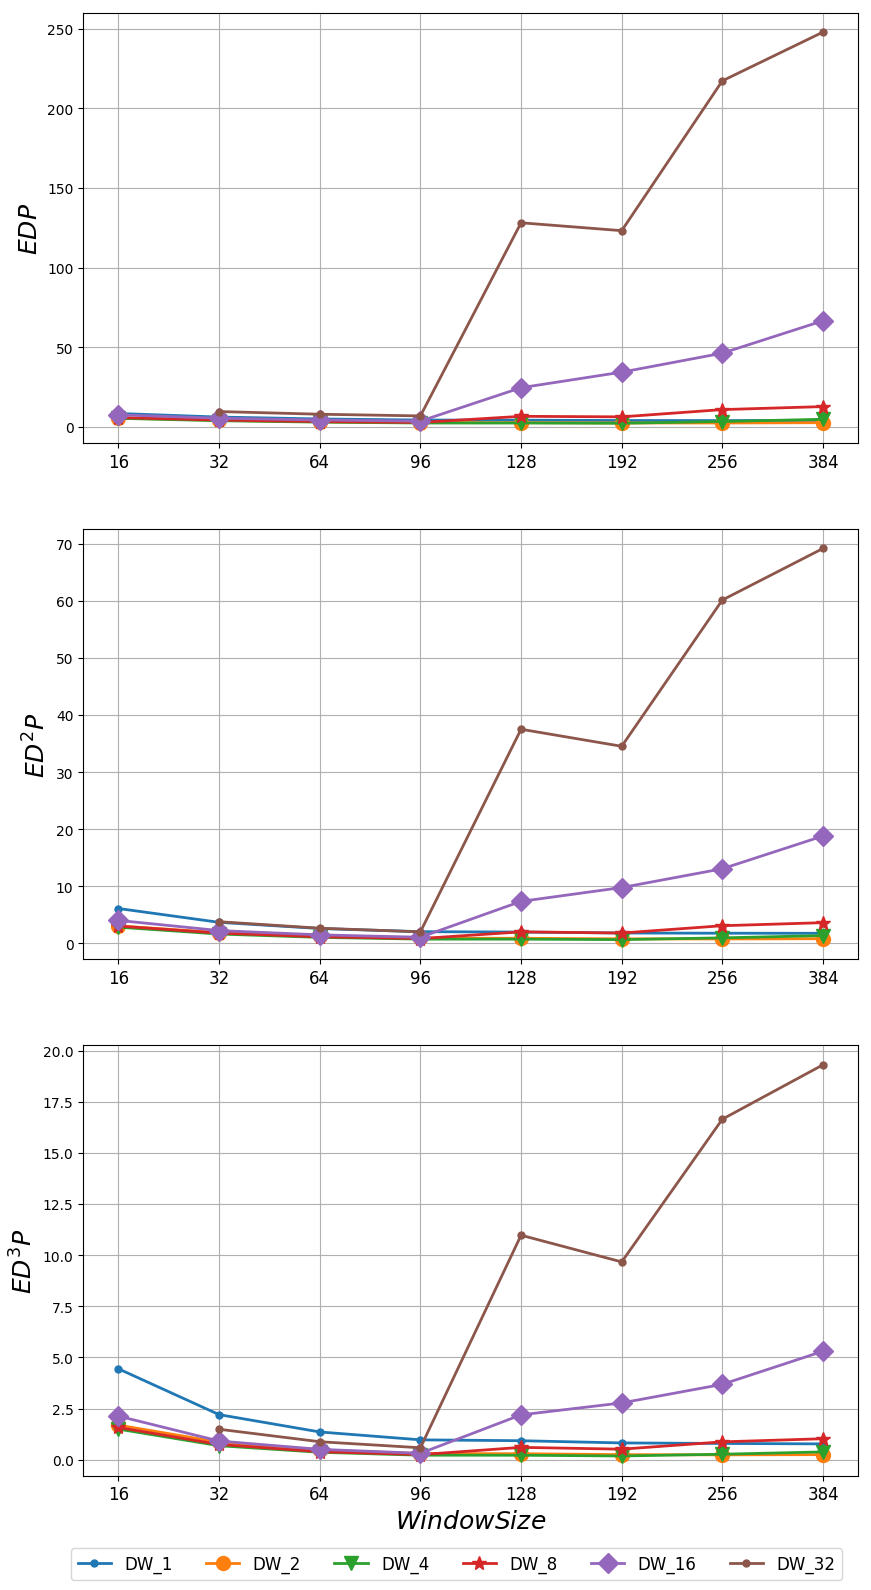
\includegraphics[width=0.7\textwidth]{./graphs/edp/cactusADM.png}
         \vspace{6mm}
      \end{center}
   \end{minipage}

   \begin{minipage}{\textwidth}
      \begin{center}
         \fbox{\textlatin{\textbf{\textit{445-gobmk}}}}\\
         \vspace{3mm}
         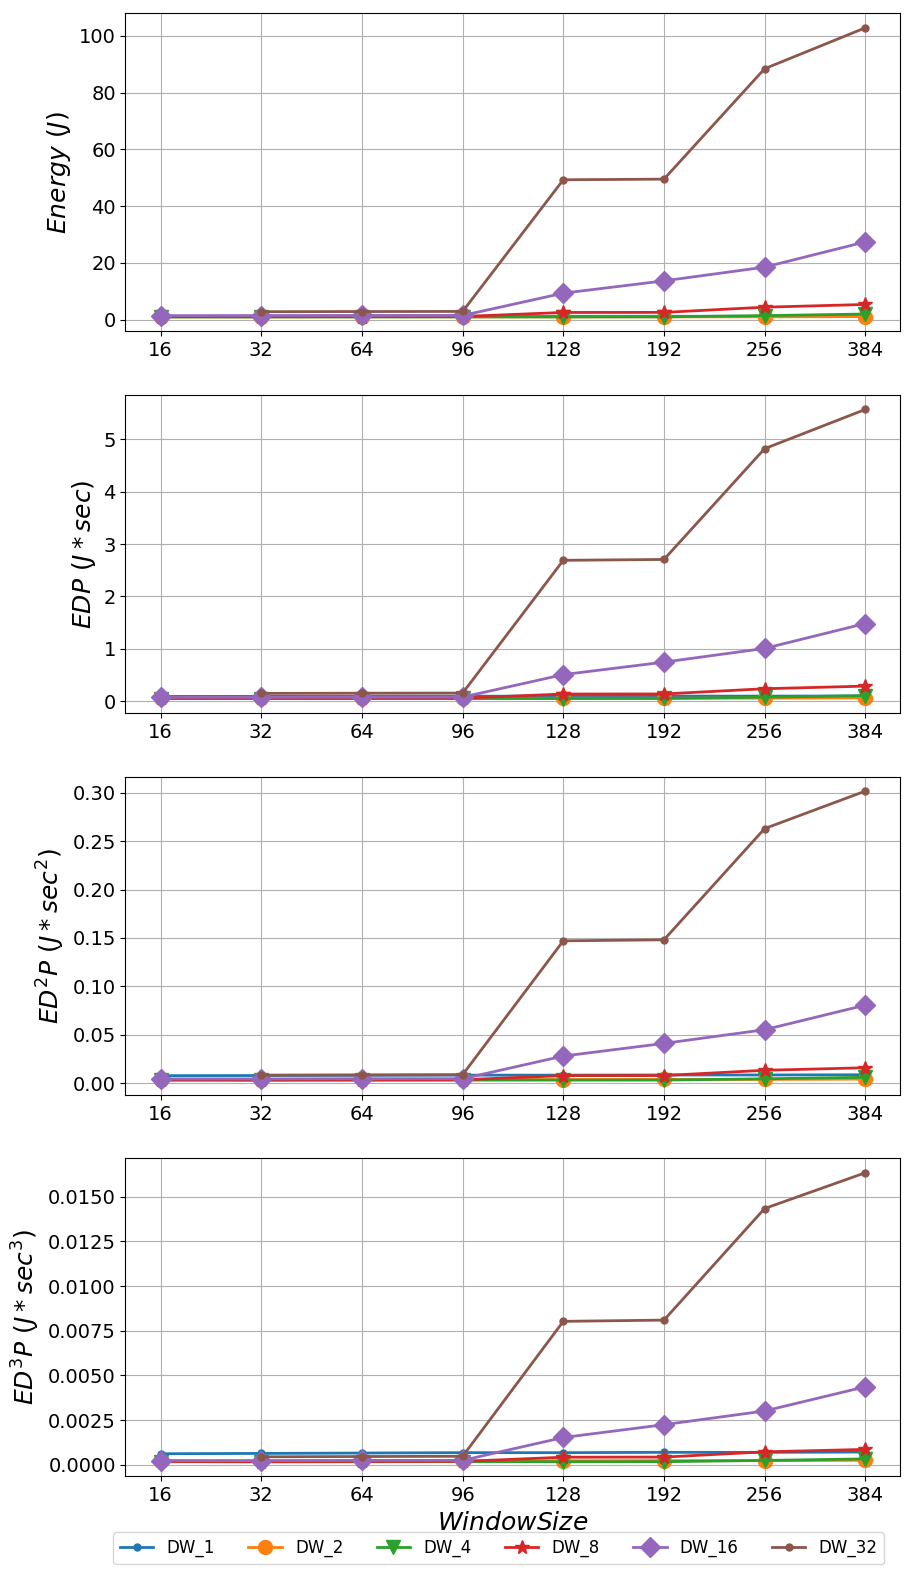
\includegraphics[width=0.7\textwidth]{./graphs/edp/gobmk.png}
         \vspace{6mm}
      \end{center}
   \end{minipage}

   \begin{minipage}{\textwidth}
      \begin{center}
         \fbox{\textlatin{\textbf{\textit{458-sjeng}}}}\\
         \vspace{3mm}
         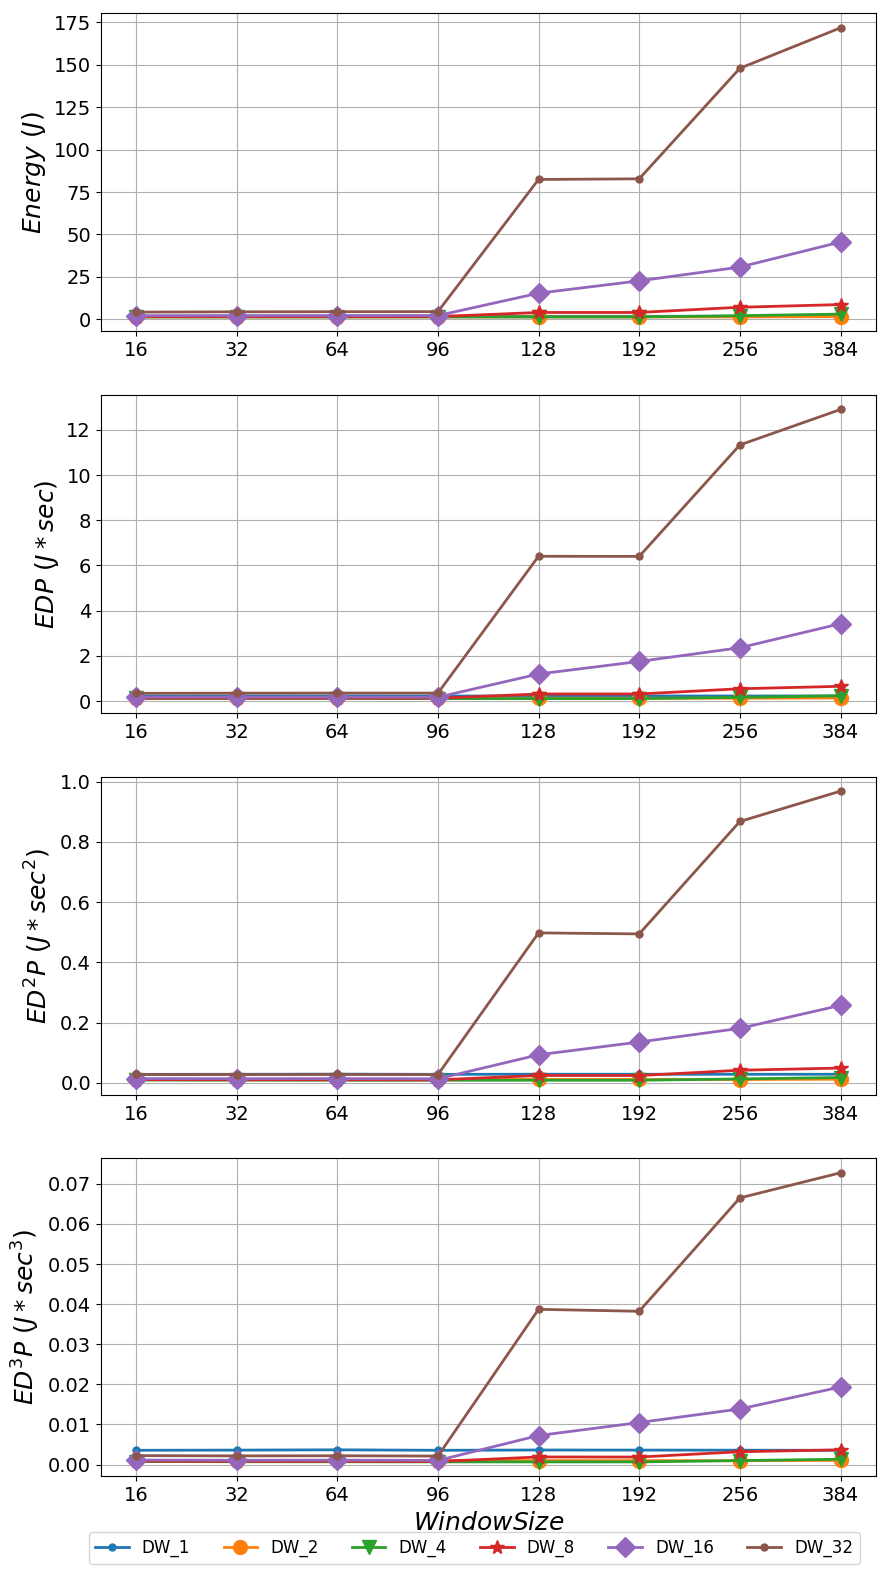
\includegraphics[width=0.7\textwidth]{./graphs/edp/sjeng.png}
         \vspace{6mm}
      \end{center}
   \end{minipage}

   \begin{minipage}{\textwidth}
      \begin{center}
         \fbox{\textlatin{\textbf{\textit{459-GemsFDTD}}}}\\
         \vspace{3mm}
         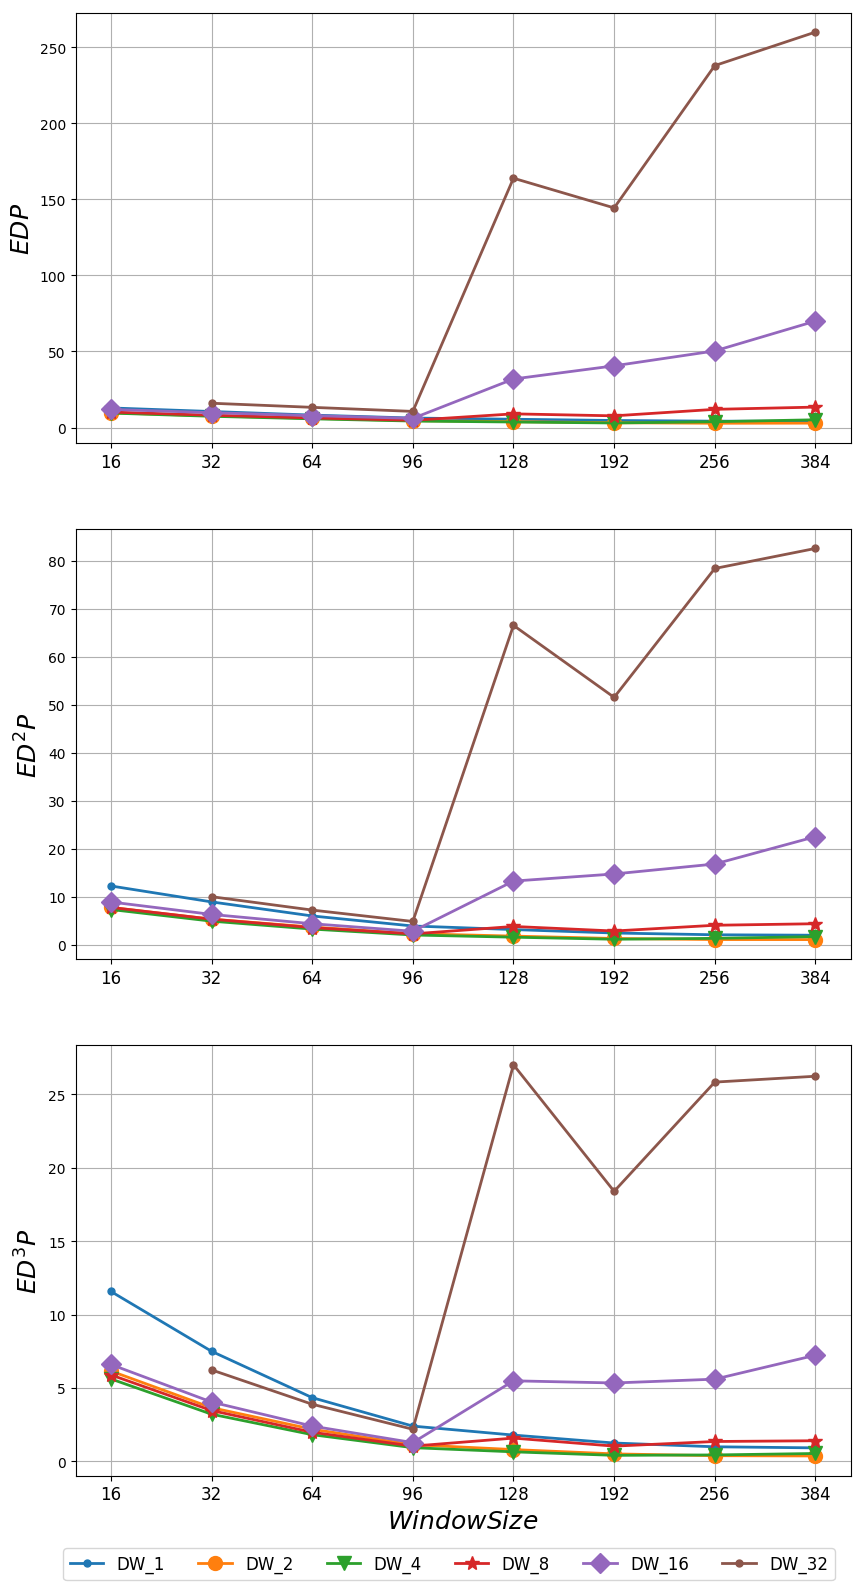
\includegraphics[width=0.7\textwidth]{./graphs/edp/GemsFDTD.png}
         \vspace{6mm}
      \end{center}
   \end{minipage}



   \paragraph{Συμπεράσματα - Σχόλια}
   Αναφορικά με το \textbf{μέγεθος} του chip, παρατηρούμε πως δεν υπάρχει
   σημαντική διαφοροποίηση μεταξύ επεξεργαστών με dispatch width 1, 2, 4 και 8
   εντολών (ανεξερατήτως window size). Συγκεκριμένα, για τις τιμές αυτές του
   dispatch width το μέγεθος είναι περί τα 100 με 150 $mm^2$ και όπως αναφέραμε
   δεν μεταβάλλεται σημαντικά καθώς το window size αυξάνει. Ωστόσο, για dispatch
   width 16 και 32 το μέγεθος αυξάνει δραματικά και επηρεάζεται από το window
   size. Αξίζει να σημειώσουμε πως για dispatch width 32 και window size 384 το
   chip αποκτά αρκετά μεγάλο μέγεθος ίσο με $1300 mm^2$.

   Ως προς την \textbf{ενέργεια} που καταναλώνεται, απεικονίζουμε στα σχετικά
   διαγράμματα τόσο την ενέργεια αλλά και τις μετρικές EDP (Energy * Runtime),
   $ED^2P$ $(Energy * Runtime^2)$, $ED^3P$ $(Energy * Runtime^3)$. Οι μετρικές
   αυτές μας δίνουν μια καλύτερη αντίληψη της ενέργειας λαμβάνοντας υπόψιν και
   την επίδοση (runtime). Συγκεκριμένα, όσο μεγαλύτερος είναι ο εκθέτης του
   runtime τόσο μεγαλύτερο το βάρος που δίνεται στην επίδοση.
   
   Παρατηρούμε ότι σε όλα τα benchmarks οι επιμέρους γραφικές για dispatch width
   1, 2, 4 και 8 είναι παραπλήσιες, και άρα η ενέργεια που καταναλώνεται είναι
   περίπου ίδια για ίδιο window size και dispatch width  1, 2, 4 ή 8.
   Παρατηρούμε επίσης πως υπάρχουν και ορισμένα benchmarks (mcf, zeus,
   cactusADM, GemsFDTD) στα οποία για τις παραπάνω τιμές dispatch width και
   μικρές τιμές window size = 16 ή 32 η ενέργεια και οι μετρικές EDP εχουν πιο
   μεγάλη τιμή σε σχέση με αυτές που αντιστοιχούν σε μεγαλύτερο window size (η
   καμπύλη είναι φθίνουσα). Η ελάχιστη ενέργεια στις περιπτώσεις αυτές φαίνεται
   να αντιστοιχεί σε window size 192 ή 256. Ωστόσο και για μεγαλύτερα window
   size δεν υπάρχει σοβαρή επίπτωση.
  
   Η επιλογή dispatch width 16 και 32 αυξάνει δραστικά την ενέργεια που
   καταναλώνεται καθώς και την επίδοση, όπως φαίνεται και από μετρικές EDP.
   Mάλιστα, για τις τιμές αυτές του dispatch widtd η ενέργεια αυξάνει
   σημαντικά καθώς αυξάνεται το window size. 
   
   Με βάση την ανάλυση αυτή αλλά και λαμβάνοντας υπόψιν την ανάλυση για την
   επίδοση στα προηγούμενα ερωτήματα, θα επέλεγα τελικώς \textbf{dispatch width
   = 4} (ή και 8) και \textbf{window size = 192 ή 256}, δεδομένου ότι γι' αυτή
   την επιλογή χαρακτηριστικών επεξεργαστή τόσο η ενέργεια και το EDP έχουν την
   ελάχιστη τους τιμή.